\chapter{ANOVA}
One-way ANOVA is a common procedure in statistics, and is related to the
simpler idea of a t-test. These classical tests were designed for particular
kinds of problems, and in this chapter we will study similar problems but
solve them from a Bayesian point of view.
We will also use these examples to discuss some issues about the choice
of prior distributions when there are more than a few parameters. When there
are only a few parameters it is usually safe to assign a vague, wide prior
to describe your initial uncertainty (unless, of course, you have more
information than that). In higher dimensions, problems can arise if you do
this. One way of getting around these problems is to use a
{\it hierarchical model}.

\section{A T-Test Example}
This example is based on one given in a 1976 article by physicist E. T. Jaynes,
called ``Confidence Intervals vs. Bayesian Intervals''. This is a very strongly
worded paper and might be an interesting read for
those who are interested in the battle between frequentist and Bayesian statistics
when the latter was making its comeback in the second half of the 20th century.
It's also where I got the crazy confidence interval example from.

Two manufacturers, $1$ and $2$, both make ``widgets'', and we are interested
in figuring out which manufacturer makes the best widgets (on average), as
measured by their lifetime. To determine this, we obtain 9 widgets from
manufacturer $1$ and 4 widgets from manufacturer $2$, and measure their
lifetimes, in days. The results are given below:
\begin{eqnarray}
x^1 &=& \{41.26, 35.81, 36.01, 43.59, 37.50, 52.70, 42.43, 32.52, 56.20\}\\
x^2 &=& \{54.97, 47.07, 57.12, 40.84\}
\end{eqnarray}
These measurements can be summarised by the means and standard deviations, which
are $42 \pm 7.48$ for group $1$ and $50 \pm 6.48$ for group $2$.
The question is: given this data, is there evidence that one of the manufacturers
is better than the other, and if so, by how much?
In classical statistics the standard procedure for this situation would be a
two sample $t$0-test. However, before we do anything I'd like you to consider
the numbers and use your intuition: what do {\it you} think about what the
evidence says?

An underlying assumption of a classical $t$-test is that the data are normally
distributed around the mean values for each group\footnote{Strictly speaking,
it's the probability distribution for the data given the parameters
that is normal, the data may or may not look normally distributed.}.
We may as well adopt this
assumption for our Bayesian model. If we call the group 1
data points $\{x^1_1, x^1_2, ..., x^1_{N_1}\}$ and the group 2 data points
$\{x^2_1, x^2_2, ..., x^2_{N_1}\}$, then the likelihood is:
\begin{eqnarray}
x^1_i &\sim& \mathcal{N}\left(\mu_1, \sigma^2\right)\nonumber\\
x^2_i &\sim& \mathcal{N}\left(\mu_2, \sigma^2\right)\label{eq:ttest_likelihood}
\end{eqnarray}
Where all the data points are independent given the parameters. Note the assumption that
the two groups have the same underlying (``population'') standard deviation $\sigma$. This is a popular
assumption in this kind of analysis but it is not necessarily well justified!
We will build our Bayesian models using this assumption, but it is not that
difficult to relax it if you want to. You could just include multiple
$\sigma$ parameters in the model,
just like how we will include the multiple $\mu$ parameters.

Instead of just one model for this situation, we will study three different
versions. Each model will have the same likelihood
as given above in Equation~\ref{eq:ttest_likelihood}, and the same prior
for $\sigma$. However, the models will all have different priors for $\mu_1$
and $\mu_2$.
We will be able to see that the choice of prior does
influence the results (of course), but in ways that make sense. Which of these
models is more appropriate in a practical situation would depend on the exact
situation. There is no ``one size fits all'' model.

\subsection{Likelihood}
To implement our model in JAGS, we can begin by specifying the likelihood
part like so:

\begin{framed}
\begin{verbatim}
    # Sampling distribution/likelihood
    for(i in 1:N1)
    {
        x1[i] ~ dnorm(mu1, 1/sigma^2)
    }
    for(i in 1:N2)
    {
        x2[i] ~ dnorm(mu2, 1/sigma^2)
    }
\end{verbatim}
\end{framed}
We have called our data arrays {\tt x1} and {\tt x2}, and we have also
assumed that the sample sizes {\tt N1} and {\tt N2} are defined, so our
{\tt data} list will need to be consistent with these choices. The parameters
we will be estimating are {\tt mu1}, {\tt mu2}, and {\tt sigma}, so we will
need to specify prior distributions for them. In the following sections, we'll
use the same prior for {\tt sigma}, so we may as well specify that now.
Let's use a log-uniform prior where $\sigma$ is between $e^{-10}$ and
$e^{10}$.

\begin{framed}
\begin{verbatim}
    # Prior for sigma
    log_sigma ~ dunif(-10, 10)
    sigma <- exp(log_sigma)
\end{verbatim}
\end{framed}

\subsection{Prior 1: Very Vague}
The last missing ingredients to finish the JAGS model are the priors for
{\tt mu1} and {\tt mu2}. For our first model, let's be really naive and assign
super-wide uniform priors.

\begin{framed}
\begin{verbatim}
    # Prior 1: Very Vague
    mu1 ~ dunif(-1000, 1000)
    mu2 ~ dunif(-1000, 1000)
\end{verbatim}
\end{framed}

At first glance, this might seem like a fairly reasonable thing to do. In many
problems, it doesn't make much difference if we just use vague priors and get
on with the calculation (as opposed to thinking really hard about the prior,
and what is actually known about the parameters).

However, this prior has a number of properties that suggest it might not be
quite right: firstly, what is the probability that $\mu_1 = \mu_2$?
In classical t-tests, the whole point is to test the hypothesis that
the two ``population means'' (parameters) are equal. However, our prior
actually implies that the probability they are equal is 0! Therefore, no matter
what data we get, the posterior probability of $\mu_1 = \mu_2$ will always be
zero.

\subsection{Prior 2: They might be equal!}
The problem with Prior 1 is that we may think $\mu_1$ might exactly equal
$\mu_2$, and Prior 1 doesn't allow for this. So here's another way we might
set up the prior. We'll start by defining the prior for $\mu_1$ as we did
before. Then, when we consider $\mu_2$, we need a way of giving it a
50\% probability of equalling $\mu_1$, and if not, then it should have
a uniform distribution between -1000 and 1000. Here is our solution. Read it
carefully and make sure you understand what this prior does.

\begin{framed}
\begin{verbatim}
    # First mean
    mu1 ~ dunif(-1000, 1000)

    # Prior on second mean, if it's different
    maybe ~ dunif(-1000, 1000)
    flag ~ dunif(0, 1)
    mu2 <- mu1 + (maybe - mu1)*step(flag - 0.5)
\end{verbatim}
\end{framed}

\subsection{Prior 3: Alright, they're not equal, but they might be {\it close}}
Prior 2 is also a little bit strange, if you think about it. If we're comparing
these two manufacturers of widgets, why would we think it is possible that the
two manufacturers are {\tt exactly} equal? Maybe we just think the parameters
$\mu_1$ and $\mu_2$ are likely to be {\it similar} in value.
In other words, we shouldn't worry so much about the
prior probablity of $\mu_1 = \mu_2$, but we should at least make sure there's
a moderate prior probability that $\mu_1 \approx \mu_2$.

One way we could do this is by applying a normal prior to both $\mu_1$ and
$\mu_2$ with some mean (let's call it the ``grand mean'')
and some standard deviation (let's call it the ``diversity'').
That way, $\mu_1$ and
$\mu_2$ would both be likely to be somewhere around the grand mean, and
they would likely be different by roughly the size of the diversity.
The challenge now seems to be the choice of appropriate values for the grand
mean and the diversity. Fortunately, we don't actually have to! What we can
do instead is apply priors for them instead.

This is our first example of a {\it hierarchical model}. In a hierarchical
model, instead of directly assigning priors to our parameters, we imagine that
we knew the values of some other parameters (called ``hyperparameters''), and
assign our prior for the parameters {\it given} the hyperparameters. Then we
assign a prior for they hyperparameters as well, to complete the model.

\begin{framed}
\begin{verbatim}
    # Hierarchical prior for the means
    # Hyperparameters
    grand_mean ~ dunif(-1000, 1000)
    log_diversity ~ dunif(-5, 5)
    diversity <- exp(log_diversity)

    # Prior for the parameters given the hyperparameters
    mu1 ~ dnorm(grand_mean, 1/diversity^2)
    mu2 ~ dnorm(grand_mean, 1/diversity^2)
\end{verbatim}
\end{framed}


Samples (obtained using JAGS) of the three priors are shown in
Figure~\ref{fig:ttest1}.
\begin{figure}[h]
\begin{center}
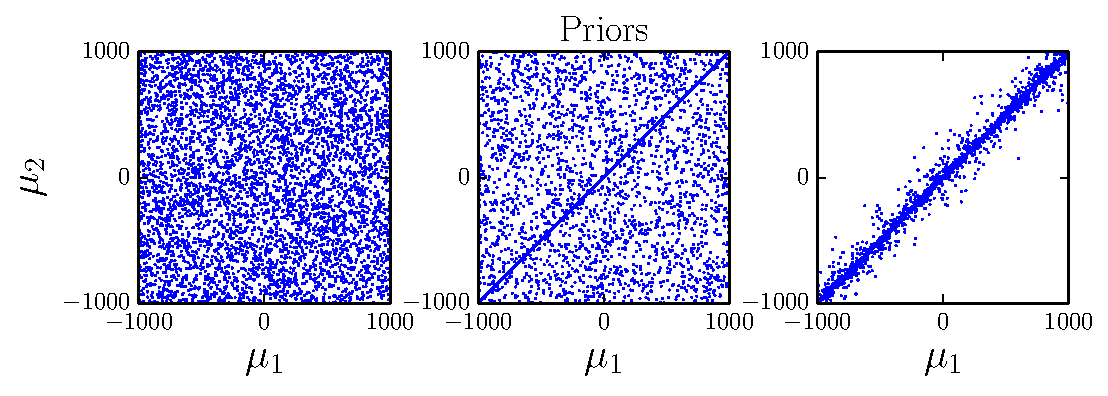
\includegraphics[scale=0.8]{Figures/ttest1.pdf}
\caption{\it The three different priors we are trying for our Bayesian
equivalent of a t-test. The first prior simply asserts a large amount of
prior ignorance about the value of the two parameters $\mu_1$ and $\mu_2$.
The second is similar but applies 50\% probability to the proposition
$\mu_1 = \mu_2$. The third prior does not allow the two parameters to be
exactly equal, but enhances the probability that they are quite similar
in value.\label{fig:ttest1}}
\end{center}
\end{figure}

The posteriors are shown in Figure~\ref{fig:ttest2}.
The inferences are different, as you would expect, and that's entirely down
to the choice of the prior. Any summaries we make will therefore depend on
which prior we want to use.
\begin{figure}[h]
\begin{center}
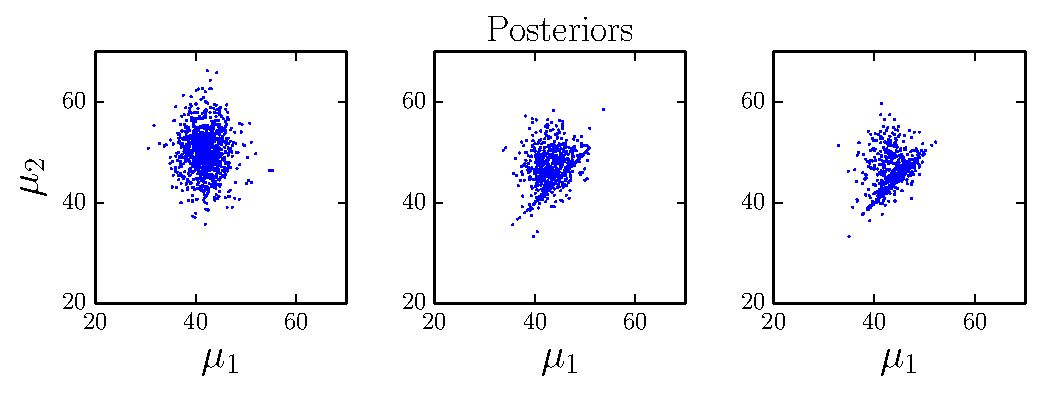
\includegraphics[scale=0.8]{Figures/ttest2.pdf}
\caption{\it The posterior distributions, given the widget data,
based on the three different priors for $\mu_1$ and $\mu_2$.\label{fig:ttest2}}
\end{center}
\end{figure}

The original question was whether manufacturer two was better, equal, or worse
than manufacturer one. We can answer that question by calculating the
posterior probabilities of $\mu_1 = \mu_2$, $\mu_1 < \mu_2$, and
$\mu_1 > \mu_2$. The results are shown in Table~\ref{tab:ttest_results}.

\begin{table}
\begin{center}
{\bf Prior Probabilities}:\\
\begin{tabular}{|l|c|c|c|}
\hline
Prior	&	$\mu_1 < \mu_2$	& $\mu_1 = \mu_2$	& $\mu_1 > \mu_2$\\
\hline
1 	&	0.5		&	0		&	0.5\\
2 	&	0.25		&	0.5		&	0.25\\
3 	&	0.5		&	0		&	0.5\\
\hline
\end{tabular}\\
{\bf Posterior Probabilities}:\\
\begin{tabular}{|l|c|c|c|}
\hline
Prior	&	$\mu_1 < \mu_2$	& $\mu_1 = \mu_2$	& $\mu_1 > \mu_2$\\
\hline
1 	&	0.946		&	0		&	0.054\\
2 	&	0.026		&	0.972		&	0.002\\
3 	&	0.693		&	0		&	0.307\\
\hline
\end{tabular}

\caption{\label{tab:ttest_results}}
\end{center}
\end{table}

Prior 1 ...
Prior 2 has bad mixing (and sensitivity to where we put the edge of the prior).
Prior 3 seems like it's what we might want in general.


\section{One Way Anova}
One-way ANOVA can be considered as a generalisation of a t-test to more than
two groups. The question is usually phrased as a test of the hypothesis that
the group means are the same, versus the alternative that there is some difference.
As we saw in the Bayesian ``t-test'', it is possible (using clever tricks) to
make a model that has some prior probability that the group means are equal.
However, this gets more tricky with multiple groups. Therefore we will build our
one-way ANOVA model in a similar way to the ``hierarchical model'' version of the
t-test model. There will be one other major difference, but it is a difference
in the way the model is coded, not a conceptual difference. In the t-test
section we used different 

The masses of starlings were measured at four locations.

\begin{figure}[ht!]
\begin{center}
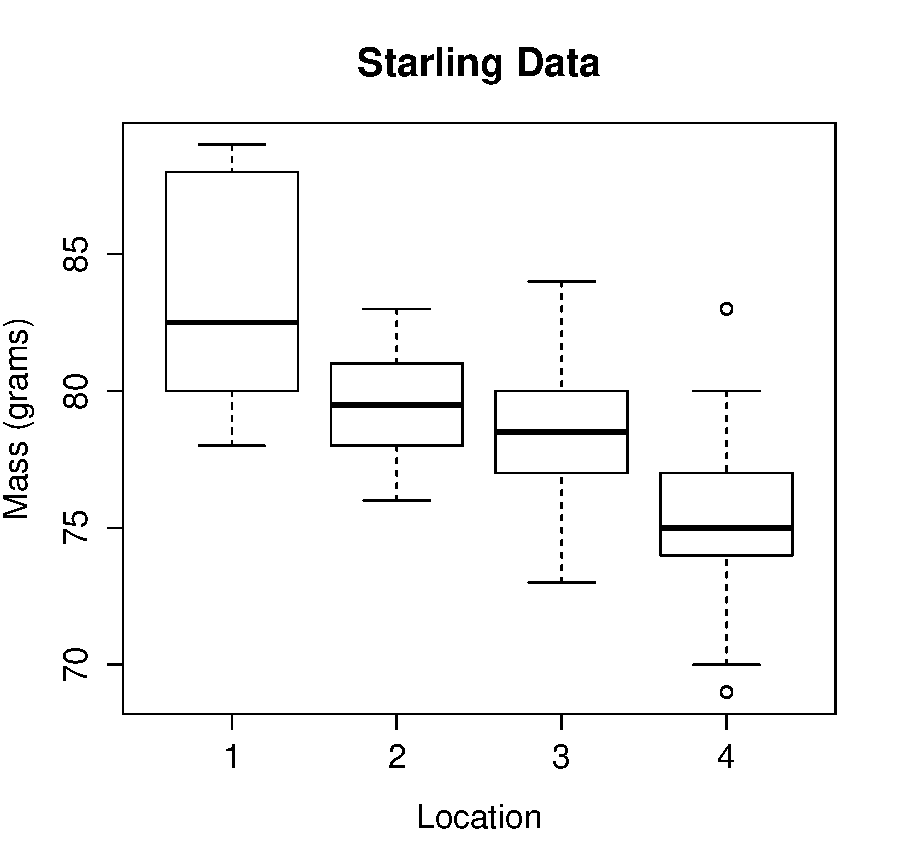
\includegraphics[scale=0.6]{Figures/starling.pdf}
\end{center}
\end{figure}


\subsection{Hierarchical Model}
The main advantage of this model is that it generalises to more than two groups
in a very straightforward way. The difference is the prior. Whereas the first
model had independent priors for the means of the groups, this version is our
first example of a {\it hierarchical model}.
\begin{framed}
\begin{verbatim}
model
{
    # Log-uniform prior for the scatter
    log_sigma ~ dunif(-10, 10)
    sigma <- exp(log_sigma)

    # Hierarchical prior for the means
    # Hyperparameters
    grand_mean ~ dnorm(0, 1/1000^2)
    log_diversity ~ dunif(-10, 10)
    diversity <- exp(log_diversity)

    # Parameters
    mu1 ~ dnorm(grand_mean, 1/diversity^2)
    mu2 ~ dnorm(grand_mean, 1/diversity^2)

    # Sampling distribution/likelihood
    for(i in 1:N)
    {
        x[i] ~ dnorm(mu[group[i]], 1/sigma^2)
    }
}

\end{verbatim}
\end{framed}


